\documentclass[letterpaper,10pt]{article}

% Construct the basic page sizes
\oddsidemargin  0.0in
\evensidemargin 0.0in
\textwidth      6.5in
\headheight     0.25in
\topmargin      0.0in
\textheight=8.5in

\usepackage{graphicx,color}

% Some text listing help for script files
\usepackage{listings}
\lstset{frame=single, captionpos=b, language=Matlab, xleftmargin=36pt, xrightmargin=36pt,
basicstyle=\ttfamily, numberstyle=\tiny, numbers=none}

% Enable verbatiminput so functional script files can be read in directly
\usepackage{verbatim}

%opening
\title{Writing a GMAT Plug-in}
\author{Darrel J. Conway\\\begin{small}Thinking Systems, Inc.\end{small}}
\date{July 24, 2008}
\begin{document}

\maketitle

\begin{abstract}
GMAT is designed to accept new user modules through shared libraries imported at run time.  This
document describes the process of building and using a GMAT plug-in.  An example is provided that
implements a modified solar radiation pressure force appropriate for use as a starting point in
building a solar sailing model.
\end{abstract}

\tableofcontents

\section{Overview}

The General Mission Analysis Tool (GMAT) contains many classes used to model spacecraft missions.
While the system contains most of the components anticipated by the project team, we also
recognized from the start that GMAT could not contain everything that every user would need.
Therefore, part of the design philosophy behind GMAT is the development of user classes that
generalize functionality in base classes that can be extended to meet future needs of the user
community.

The user configurable components of GMAT are all derived from a general purpose base class,
GmatBase, which defines interfaces used throughout the system to access common properties of the
user classes.  This base class defines a framework used by GMAT's engine to manage the objects used
when modeling a mission.

Classes derived from GmatBase are specialized to model different aspects of the mission.  Classes
located deeper in the GmatBase class hierarchy are, in general, more specialized than those at the
higher levels.  Details of GMAT's class structure can be found in the GMAT Architectural
Specification\cite{ArchSpec}, or by running GMAT's source code through the Doxygen source code
documentation generator\cite{Doxygen}.  The classes derived from GmatBase are called GMAT's user
classes.  GMAT also contains classes that do not share this ancestor; those components make up the
elements of the engine, user interfaces, and other elements of GMAT's framework that provides the
infrastructure for the system.

Builds of GMAT made using development source code after June 25, 2008 \footnote{The development code
for this capability will be merged into the trunk code when the next merge occurs.} have the ability
to load shared libraries at run time and retrieve new user objects from these libraries. The
approach taken for this capability was built on a prototype extension implemented at Thinking
Systems in April, 2008 to meet some specific mission needs and documented as an extension to
GMAT\cite{pluginProp}. This document explains how to use the plug-in extensions to add new
capabilities to GMAT.  A specific example -- the addition of a new force for GMAT's force model --
is described in some detail, with emphasis on the features necessary for incorporation into GMAT at
run time.

We'll begin by looking at the steps needed to construct a GMAT plug-in.  Once these steps have been
described, the design of the example plug-in code -- a basic solar sail model for GMAT's force
model -- is described, along with descriptions of the pieces needed to incorporate the new model
through the plug-in interface.  Finally, the steps needed to tell GMAT about the new plug-in are
presented.  The document closes with appendices that describe details of the development process for
Eclipse users, and that contain full source code listings for the six files that comprise the
plug-in.

\section{Plug-in Programmatic Requirements}

GMAT's Plug-in capabilities apply to the classes derived from the GmatBase class.  Instances of
these classes are constructed using GMAT's Factory subsystem.  Plug-in authors capitalize on this
design by creating custom factories designed to support the new components that they are adding to
the system.  A GMAT plug-in is a shared library, linked against a shared library build of GMAT's
base code, that contains the class code for the new capability, one or more supporting Factory for
the new components, and a set of three C-style interface functions that are accessed by GMAT to
load the plug-in.  Each of these plug-in elements is introduced in this section, starting from the
build requirements for GMAT, proceeding through the interface functions and factory requirements,
and finishing with the actual new component that is being added.  The next section of this document
describes a sample plug-in of to illustrate the process.

\subsection{Building GMAT for Plug-in Use}

GMAT plug-ins create classes that are derived from classes in GMAT's base code.  The plug-in needs
to be linked against that code in order to use the capabilities of the base classes, and to build
the complete derived objects.  In order to do this, the plug-in library needs to be linked against
the base code that will be run when GMAT runs.  There are two ways this requirement can be
accomplished.  The code can be built with all of the required classes as part of the plug-in
library.  That approach makes the plug-in much larger than necessary; in general, GmatBase
subclasses need the code from the utility and foundation folders, the folders related to the type
of subclass that is being built, and all of the referenced classes used by the members of its
hierarchy.  In addition, these elements need to stay synchronized with GMAT's base code as new
features are implemented and as anomalies are corrected in the base code.

The preferred approach to plug-in development is to build GMAT's base code as one or more shared
libraries.  GMAT's build control file, BuildEnv.mk, has a setting for this option.  If you add this
line to the file:

\begin{quote}
\begin{verbatim}
SHARED_BASE = 1
\end{verbatim}
\end{quote}

\noindent and then clean and build GMAT, the make files will build the base code as a shared library
-- named libGmatGui -- that can be used for plug-in development.  Once you have built GMAT this
way, you are ready to start coding your plug-in.

\subsection{The Plug-in Interface Functions}

GMAT accesses new user classes contained in plug-in libraries by calling three methods in the
plug-in: GetFactoryCount(), GetFactoryPointer(), and SetMessageReceiver().  These functions are
used as the entry point into the plug-in components.  They are defined as follows:

\begin{itemize}
\item \texttt{Integer GetFactoryCount()}:  This function reports the number of Factory classes
that are contained in the plug-in.  The current implementation of GMAT requires that factories only
support a single core type because of an implementation limitation in the FactoryManager, so larger
plug-in libraries may need more than one supporting factory.
\item \texttt{Factory* GetFactoryPointer(Integer index)}:  This function retrieves Factory pointers
from the plug-in.  Once GMAT know the number of factories in the library, it calls this function to
retrieve the contained factories one at a time.
\item \texttt{void SetMessageReceiver(MessageReceiver* mr)}:  Messages posted in GMAT are all sent
to a MessageReceiver.  This function is used to set the MessageReceiver for a plug-in.

\begin{quote}
\begin{small}Note: The design that required this method incorporated base code in the plug-in
library.  Now that the base code can -- and should be -- built as a shared library, this function
may no longer be needed, and may be removed at a later date.\end{small}
\end{quote}
\end{itemize}

\noindent The code in Section~\ref{sec:InterfaceCode} shows one implementation of these methods.

\subsection{The Custom Factory}

GMAT's Factory subsystem is described in some detail in the Architectural
Specification\cite{ArchSpec}.  GMAT uses this subsystem to create user objects that are needed to
run a mission.  The class diagram for the subsystem is shown in Figure~\ref{fig:FactorySubsystem}.

\begin{figure}[tb]
\begin{center}
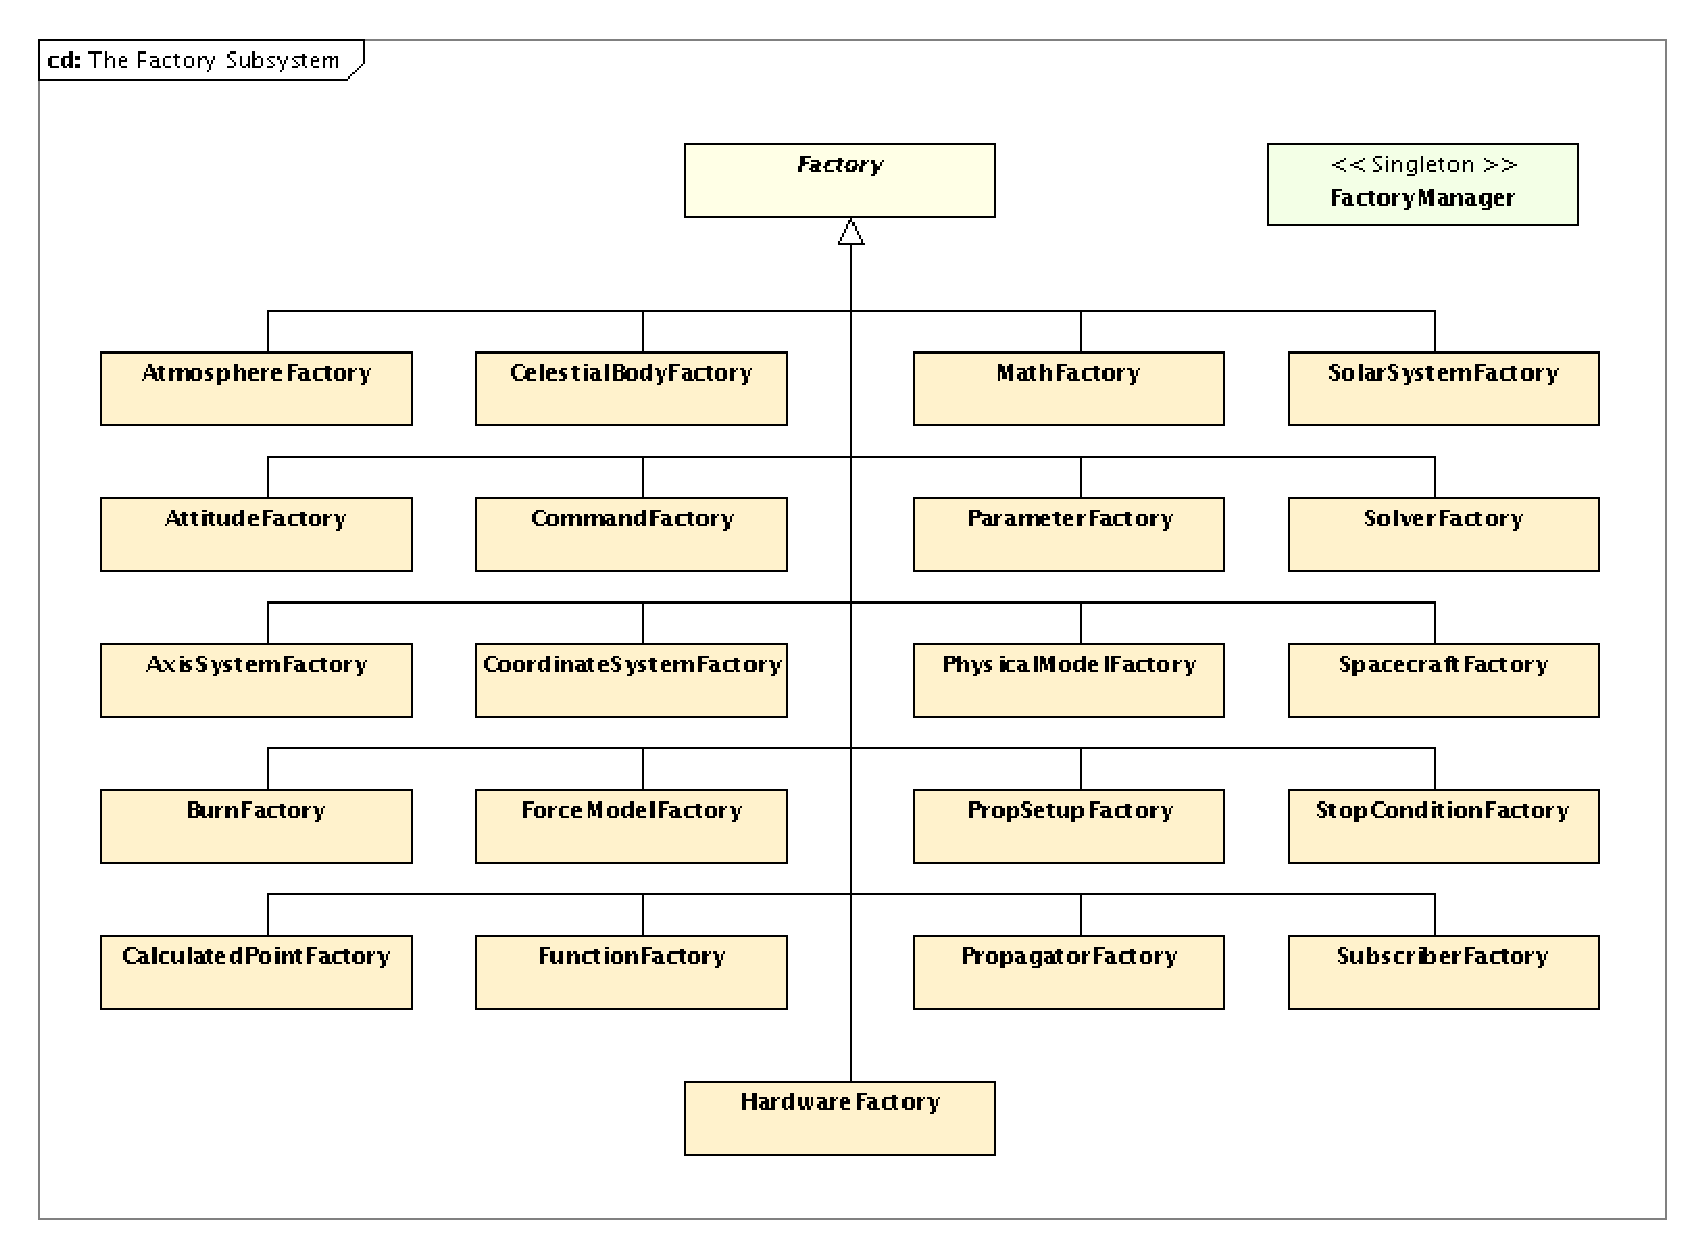
\includegraphics[bb=0 0 800 586,scale=0.5,clip]
{Images/TheFactorySubsystem.eps}
\caption{\label{fig:FactorySubsystem} The Factory Subsystem}
\end{center}
\end{figure}

The Factory base class defines the interface used to create user objects.  It includes subclass
specific interfaces for the core user class types, as can be seen from this portion of the class
definition:
\begin{quote}
\begin{small}
\begin{verbatim}
class GMAT_API Factory
{
public:
   // method to return objects as generic type
   virtual GmatBase*        CreateObject(const std::string &ofType,
                                         const std::string &withName = "");

   // methods to return objects of specified types
   virtual SpaceObject*     CreateSpacecraft(const std::string &ofType,
                                             const std::string &withName = "");
   virtual Propagator*      CreatePropagator(const std::string &ofType,
                                             const std::string &withName = "");
   virtual ForceModel*      CreateForceModel(const std::string &ofType,
                                             const std::string &withName = "");
   virtual PhysicalModel*   CreatePhysicalModel(const std::string &ofType,
                                                const std::string &withName = "");
   virtual PropSetup*       CreatePropSetup(const std::string &ofType,
                                            const std::string &withName = "");
   virtual Parameter*       CreateParameter(const std::string &ofType,
                                            const std::string &withName = "");
   virtual Burn*            CreateBurn(const std::string &ofType,
                                       const std::string &withName = "");
   virtual StopCondition*   CreateStopCondition(const std::string &ofType,
                                                const std::string &withName = "");
   virtual CalculatedPoint* CreateCalculatedPoint(const std::string &ofType,
                                                  const std::string &withName = "");
   virtual CelestialBody*   CreateCelestialBody(const std::string &ofType,
                                                const std::string &withName = "");
   virtual SolarSystem*     CreateSolarSystem(const std::string &ofType,
                                              const std::string &withName = "");
   virtual Solver*          CreateSolver(const std::string &ofType,
                                         const std::string &withName = "");
   virtual Subscriber*      CreateSubscriber(const std::string &ofType,
                                             const std::string &withName = "",
                                             const std::string &fileName = "");
   virtual GmatCommand*     CreateCommand(const std::string &ofType,
                                          const std::string &withName = "");
   virtual AtmosphereModel* CreateAtmosphereModel(const std::string &ofType,
                                                  const std::string &withName = "",
                                                  const std::string &forBody = "Earth");
   virtual Function*        CreateFunction(const std::string &ofType,
                                           const std::string &withName = "");
   virtual Hardware*        CreateHardware(const std::string &ofType,
                                           const std::string &withName = "");
   virtual AxisSystem*      CreateAxisSystem(const std::string &ofType,
                                             const std::string &withName = "");
   virtual CoordinateSystem* CreateCoordinateSystem(const std::string &ofType,
                                                    const std::string &withName = "");
   virtual MathNode*        CreateMathNode(const std::string &ofType,
                                           const std::string &withName = "");
   virtual Attitude*        CreateAttitude(const std::string &ofType,
                                           const std::string &withName = "");
   ...
\end{verbatim}
\end{small}
\end{quote}

\noindent When you have decided what type of new component you will be implementing, select the
appropriate factory method from this group and implement it to call your component's constructor.
Each of the factory classes shown in Figure~\ref{fig:FactorySubsystem} are available for browsing
in the src/base/factory folder of GMAT's source tree, so you should be able to select an
appropriate Factory as a starting point for your custom Factory.  Section~\ref{sec:FactoryCode}
shows sample code for a Factory supporting a new PhysicalModel class.

\subsection{The New Feature}

The purpose of all of the support code described above is, of course, the implementation of a new
user component.  GMAT provides a rich set of classes that can be used as a starting point for your
new component.  If you use an existing class as your base class for the new feature, you'll find
that there is support for most or all of the plug-in component in the core GMAT engine already,
significantly reducing your integration efforts\footnote{The GMAT developers have endeavored
to keep the internal interfaces into GMAT as generic as possible.  However, it may be that we
have overlooked a feature that is critical yo your new component.  If you think that may have
happened, please send additional interface requests to the GMAT team so that we can provide
assistance and, if needed help to update GMAT's interfaces to address your needs.}.  The next
section describes the design and implementation of one such component -- a custom force used in
GMAT's force model.

\section{An Example}

This section presents the design for a complete GMAT plug-in library.  The example shown here
is a new force for the force model.  The new force used for this example is a directed solar
radiation pressure force, appropriate for solar sailing.  Appendix~\ref{sec:SourceListing} contains
the complete source code listing for this plug-in library.

For the purposes of this example, the spacecraft attitude will be used to calculate the direction
of the normal to the reflecting surface, and thus the direction of of the force vector.  More
specifically, for this example the spacecraft's x-axis, as specified by its attitude, will be
treated as the normal, $\hat \textbf{n}$, to the surface that the light hits.  The spacecraft's
coefficient of reflectivity, $1 <= C_r <= 2$, determines the amount of light that reflects off of
the spacecraft; $C_r = 1$ means that all of the incident light is absorbed, while $C_r = 2$ means
that the light is all reflected.

The following sections define the new force, describe the class used to model the force, and then
present the code needed to add the new force to GMAT using the plug-in architecture.

\subsection{The Physics of the SolarSail Model}

We'll begin by describing the model implemented in the code.  The vector from the spacecraft to the
Sun, $e_s$, makes an angle $\theta$ with the surface normal $\hat \textbf{n}$.  The absorbed
radiation applies a force $f_a$ directed opposite to the sun vector.  The reflected radiation
applies a force directed anti-parallel to the normal vector, $\hat \textbf{n}$.

The magnitude of each of these forces is equal to the incident radiation pressure $P_r$ multiplied
by the incident surface area, $A$, and then adjusted to take into account the amount of light
reflected or absorbed.  The force for absorbed light is given by

\begin{equation}\label{eq:absorbedLight}
\textbf{F}_{abs} = -(1 - \varepsilon) P_r A \cos(\theta) \hat{\textbf{e}}_s
\end{equation}

\noindent while that of the reflected light is given by

\begin{equation}\label{eq:reflectedLight}
\textbf{F}_{ref} = -2 \varepsilon P_r A \cos^2(\theta) \hat{\textbf{n}}
\end{equation}

\noindent The constant $\varepsilon$ in these equations is the percentage of the incident light
that is reflected from the surface, and is related to the coefficient of reflectivity through the
equation

\begin{equation}\label{eq:CrEpsilon}
\textbf{C}_r = 1 + \varepsilon
\end{equation}

\noindent Finally, the factor of 2 in equation~\ref{eq:reflectedLight} accounts for the
reflectance effect of Newton's third law.  The cosine term in this equation is squared because the
reflected light applies its force exclusively in the anti-normal direction; the force components
parallel to the reflecting surface from the incoming and outgoing light cancel out.

The incident radiation pressure, $P_r$, is a function of the distance from the Sun to the
spacecraft.  Spacecraft closer to the Sun experience a larger incident radiation pressure than those
further away.  This effect follows an inverse square relationship; if the solar radiation pressure
at one astronomical unit from the Sun, $R_{AU}$, is written as $P_{AU}$, the radiation pressure at
an arbitrary distance $r_s$ is given by

\begin{equation}
P_r = P_{AU} \left(\frac{R_{AU}}{r_s}\right)^2
\end{equation}

Putting all of these pieces together, the force implemented in this plug-in is given by

\begin{equation}
\textbf{F}_{sail} = -P_{AU} \left(\frac{R_{AU}}{r_s}\right)^2 A \cos\theta \{(1 -
\varepsilon) \hat{\textbf{e}}_s + 2 \varepsilon \cos\theta \hat{\textbf{n}}\}
\end{equation}

GMAT's equations of motion are expressed in terms of derivatives of the position vectors.  That
means that the function that models a force in GMAT, \texttt{GetDerivatives()}, needs to express
the effect of the force in terms of an acceleration.  The Spacecraft model contains a reflectivity
coefficient, $C_r$, which matches the coefficient in equation~\ref{eq:CrEpsilon}.  Using
equation~\ref{eq:CrEpsilon} and the relationship $\textbf{F} = m\textbf{a}$, the resulting
acceleration is

\begin{equation}
\textbf{a}_{sail} = -P_{AU} \left(\frac{R_{AU}}{r_s}\right)^2 \frac{A}{m} \cos\theta \{(2 -
C_r) \hat{\textbf{e}}_s + 2 (C_r - 1) \cos\theta \hat{\textbf{n}}\}
\end{equation}

\noindent This equation is encapsulated in the class, SolarSail, described below.

\subsection{The SolarSail Class}

GMAT's force model classes are all implementations of a base PhysicalModel class.  The SolarSail
plug-in uses many of the features and structures already implemented in the SolarRadiationPressure
class, one of the members of the force model subsystem.  The SolarSail class uses its own factory,
implemented as the Factory component of the plug-in library.  These additions are shown in the
ForceModel class hierarchy, shown in Figure~\ref{figure:ForceModelWithSail}.

\begin{figure}[tb]
\begin{center}
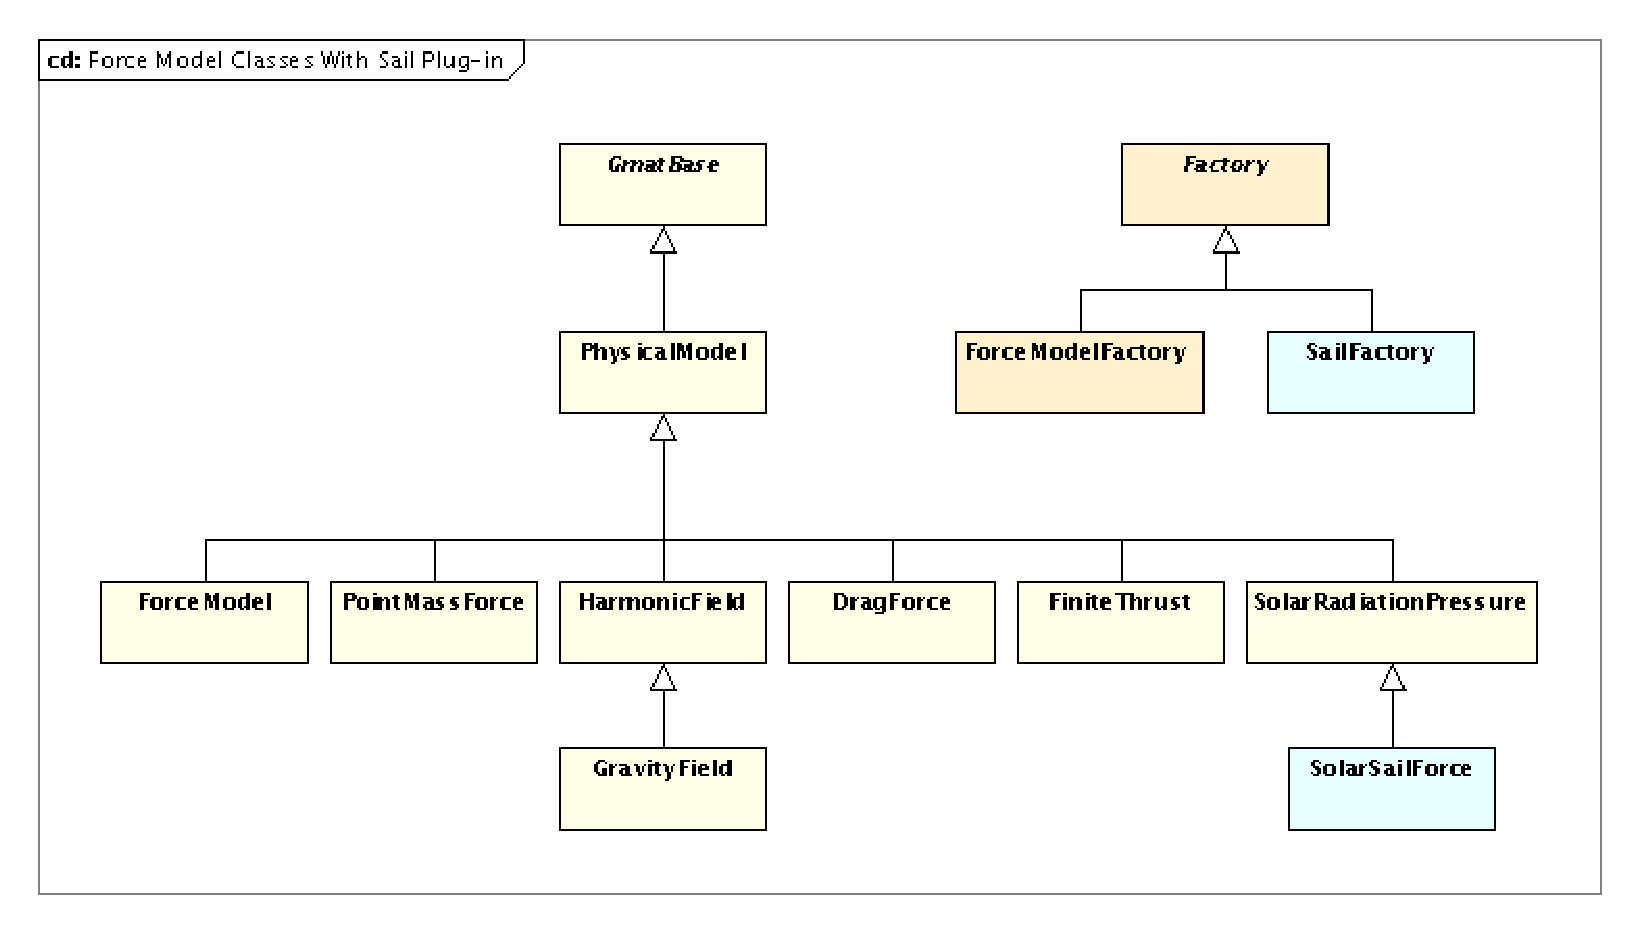
\includegraphics[bb=0 0 770 430,scale=0.5,clip]
{Images/ForceModelClassesWithSailPlugin.eps}
\caption[The Solar Sail Model Components]{\label{figure:ForceModelWithSail} The Solar Sail Model
Components.  The plug-in components are shown in blue.}
\end{center}
\end{figure}

The solar sail force uses many of the same calculations as are performed for GMAT's solar radiation
pressure model.  For that reason, the SolarSailForce class is derived from the
SolarRadiationPressure class.  The new class does need to implement a different acceleration model,
so it overrides the GetDerivatives() method to provide accelerations as described above.  It also
provides implementations for the four C++ default methods: the constructor, copy constructor,
destructor, and assignment operator.  The new force has data structures that need to be
initialized, so the Initialize() method is overridden (and calls the
SolarRadiationPressure::Initialize() method internally).  GMAT's ForceModel class contains a
method, IsUserForce(), which is called to determine how to handle scripting for forces added by
users.  This method is overridden to report the new force as a user force.  Finally, the Clone()
methods is overridden so that GMAT can make copies of the new force from a GmatBase pointer.

The full source code for the SolarSailForce class is included in Appendix~\ref{sec:SourceListing},
Section~\ref{sec:SailCode}.

\subsection{The SailFactory and Interface code}

The SailFactory is used to create new instances of the SolarSailForce.  The code -- shown in
Section~\ref{sec:FactoryCode} -- is identical to many of the core factories found in GMAT's
src/base/factory file folder.  There are three sections specific to the SolarSailForce: the
CreatePhysicalModel() method:

\begin{quote}
\begin{verbatim}
PhysicalModel* SailFactory::CreatePhysicalModel(const std::string &ofType,
                                    const std::string &withName)
{
   if (ofType == "SailForce")
      return new SolarSailForce(withName);

   return NULL;
}
\end{verbatim}
\end{quote}

\noindent and the code in the constructor and copy constructor that populates the list of creatable
object names.  That code has this form:

\begin{quote}
\begin{verbatim}
   if (creatables.empty())
   {
      creatables.push_back("SailForce");
   }
\end{verbatim}
\end{quote}

\noindent The rest of the factory code fills out the required elements: the constructors,
assignment operator, and destructor, as required in GMAT's coding standards\cite{codeStandards}.

The code in the interface functions is nearly as transparent.  There are three C-style functions
that are used in the plug-in implementation, shown in Listing~\ref{sec:InterfaceCode}.  The
GetFactoryCount() method returns the number of factories in the plug-in -- one (1) for this
example. GetFactoryPointer() creates an instance of the SailFactory and returns it to GMAT when it
is called with an input index of 0 (indicating the first factory in the plug-in).
SetMessageReceiver() is used by GMAT to ensure that the MessageReceiver pointer in the plug-in is
set to the active MessageReceiver for the executable\footnote{SetMessageReceiver() may be removed in
future builds. Early versions of the plug-in code required independent builds of the
MessageInterface code, and needed to set the MessageReceiver pointer for that code for each plug-in.
 When plug-in libraries are built that use the shared library base code for GMAT, that step is not
necessary.}

Once the code described above is in place, it can be compiled into a shared library that meets
GMAT's plug-in requirements.  The steps needed for the compilation process for Eclipse users are
described in Appendix~\ref{sec:eclipseConfiguration}.

\subsection{Adding the Plug-in to GMAT}

Once you have built the plug-in library described above, place the resulting code in the folder
that contains your GMAT executable.  The plug-in will become available in GMAT if you add a line to
your GMAT startup file identifying the library as a plug-in.  The required line looks like this for
a plug-in named libSolarSail:

\begin{quote}
\begin{verbatim}
PLUGIN               = libSolarSail
\end{verbatim}
\end{quote}

\noindent (The actual plug-in file name depends on your operating system -- on Windows, the file
name would be ``libSolarSail.dll''; on Linux, it would be ``libSolarSail.so'', and on Mac,
``libSolarSail.dylib''.)

Once this line is in place in your startup file, GMAT will attempt to load the plug-in when it is
started.

\section{Summary}

This document described the code necessary to construct a GMAT plug-in.  It described the three
core elements of a plug-in: the new functionality, the supporting factory, and the interface code
used to load the plug-in features.  An example, implemented in the code in the appendices, was
described that illustrated the addition of a force for GMAT's force model.  Finally, the steps
needed to tell GMAT about the new functionality were provided.

Please feel free to contact the author of this document with questions or requests for
clarification by sending an e-mail to djc@thinksysinc.com.

\appendix

\section{\label{sec:eclipseConfiguration}Eclipse Configuration for the Solar Sail Plug-in}

This appendix outlines the steps used to build the plug-in using Eclipse.

\subsection{Create the Project}

\begin{enumerate}
\item Open Eclipse
\item Right-click in the Project Explorer, and add a New -$>$ C++ Project.
\item On the new project dialog, set the project name to ``SolarSail'' and the project type to
``Shared Library.''
\item Press the ``Next'' button.
\item Set the desired configurations.  (I use the defaults.)
\item Press the ``Finish'' button.
\end{enumerate}

This gives you a project to use to build the plug-in library.  Next you need to configure the
project to use the GMAT shared base library.

\subsection{Configure the project}

\begin{enumerate}
\item Right click on the SolarSail node, select ``New -$>$ Folder,'' and add a directory named
``src''
\item Add three folders under the src folder, named ``plugin,'' ``sail,'' and ``factory.''  These
are the folders that will contain the six source files needed for the plug-in.
\item Place the source files in the corresponding folders.  The source files are available on
GMAT's Wiki pages.
\end{enumerate}

The next step is configuring Eclipse so that the C++ compiler and linker know where to find the
header files and libraries needed to build the plug-in.

\begin{enumerate}
\item Right-click on the project node in the Project Explorer, and select the ``Properties'' option.
\item On the Properties dialog, select the ``C/C++ Build | Settings'' option from the panel on the
left.
\item On the right panel, select ``GCC C++ Compiler | Directories.''
\item Press the ``Add'' button on the Include paths toolbar.
\item Press the ``Workspace...'' button on the ``Add directory path'' pop-up window, and navigate
to the SolarSail/src/factory folder on the ``Folder selection'' pop-up dialog.  Press the OK button
to accept this path. Then press the OK button on the ``Add directory path'' dialog to send the path
to the Eclipse settings panel.
\item Repeat the previous step to add the plugin and sail directory folders to your configuration.
\item Use this procedure to add the following folders from your GMAT build to the include
directories:
\begin{itemize}
\item src/base/include
\item src/base/util
\item src/base/foundation
\item src/base/factory
\item src/base/forcemodel
\item src/base/solarsys
\item src/base/spacecraft
\item src/base/coordsys
\item src/base/attitude
\end{itemize}
\end{enumerate}

$<$Add Windows specifics -- linking against the dll, and anything else uncovered when testing
there.$>$

This completes the steps needed to build the plug-in.  Right-click on the project node and select
the ``Build Project'' option.  Eclipse will build a new shared library for you, and place it in the
Debug folder.  Move that library into the GMAT executable folder and edit the startup file to use
the new code.

\section{\label{sec:SourceListing}Source Code for the Plug-in}

This section contains the SolarSail plug-in code in its entirety.  The plug-in is built using six
files, grouped as a header file and implementation.  The generic interface functions are
implemented in the plugin/GmatPluginFunctions code.  The Factory supporting the new plug-in class
in implemented in the factory/SailFactory code.  The sail/SolarSailForce code implements the new
force.

\subsection{\label{sec:InterfaceCode}The Plug-in interface Code}

\subsubsection{src/plugin/GmatPluginFunctions.hpp}

\verbatiminput{Code/GmatPluginFunctions.hpp}

\subsubsection{src/plugin/GmatPluginFunctions.cpp}

\verbatiminput{Code/GmatPluginFunctions.cpp}

\subsection{\label{sec:FactoryCode}The Factory Code}

\subsubsection{src/factory/SailFactory.hpp}

\verbatiminput{Code/SailFactory.hpp}

\subsubsection{src/factory/SailFactory.cpp}

\verbatiminput{Code/SailFactory.cpp}

\subsection{\label{sec:SailCode}The Solar Sail Force Code}

\subsubsection{src/sail/SolarSailForce.hpp}

\verbatiminput{Code/SolarSailForce.hpp}

\subsubsection{src/sail/SolarSailForce.cpp}

\verbatiminput{Code/SolarSailForce.cpp}

\begin{thebibliography}{10}
\bibitem{ArchSpec} The GMAT Development Team, \textit{The GMAT Architectural Specification}, (March
2008).

\bibitem{Doxygen} Dimitri van Heesch, \textit{Doxygen}, Available for free download at
http://www.stack.nl/~dimitri/doxygen/.

\bibitem{pluginProp} Darrel J. Conway, \textit{An Approach to Plug-in Coding in GMAT}, (May 2008).

\bibitem{codeStandards} Wendy Shoan and Linda Jun, \textit{C++ Coding Standards and Style Guide},
as modified for the GMAT project (October 2008).

\end{thebibliography}

\end{document}
